% Proposal for the features and scoring and stuff of my senior project.
\documentclass{article}
\title{Senior Project Presentation}
\author{Steve Jarvis}
\date{\today}
% Disables chapter and section numbering
\setcounter{secnumdepth}{-1} 
\usepackage[pdftex]{graphicx}
\usepackage{listings}

\begin{document}
\maketitle

\section{What I Learned...}

\subsection{What's a Neural Network?}

    \paragraph{}A neural network is a general machine learning tool that can be 
    used to learn a large variety of data sets. A neural network is named so 
    because of its inspiration: biological neurons in the brain! A conventional
    artificial neural network learns by making an estimate, getting feedback, and 
    adjusting the priority given to all its connections (neurons) in such a way 
    that it inches towards the correct answer.

    \paragraph{}The simplest neural network is one consisting of two layers. A 
    weight connects each node in the first layer to each node in the second layer.
    Such a network could be trained to learn learn logical OR. Imagine three input 
    nodes and two output, with the bottom left representing false and the bottom 
    right true. When inputting bits representing logical OR, the network should 
    yield output representing true (in this case, a positive value in the right
    output node and negative in the left output node). See 
    Figure~\ref{basicnetwork} on  page~\pageref{basicnetwork} for an 
    illustration.

    \paragraph{}An important consideration for this sample network is its limited 
    learning ability. A two-layer network can only learn linearly separable 
    functions; equations whose positive and negative results, when graphed, can 
    be partitioned by a single line. More complex functions require deeper networks
    to learn, although the complexity increases quickly. With only a single extra 
    layer (and ~200 nodes per layer) the neural net used in this project was able 
    to achieve 93 percent accuracy on the MNIST Database of Handwritten 
    Digits\footnote{http://yann.lecun.com/exdb/mnist/}.

    \begin{figure}
        \centering
        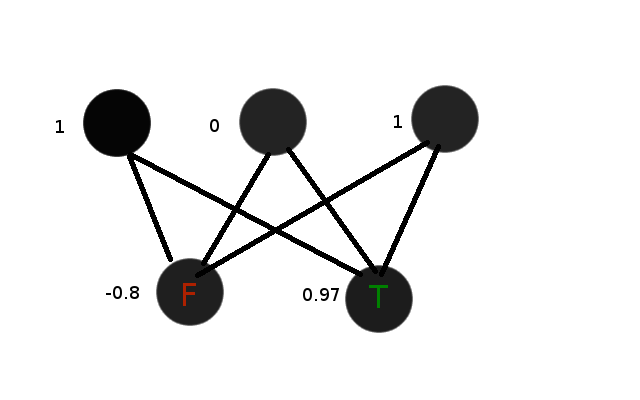
\includegraphics[scale=0.4]{images/perceptron.png}
        \caption{The top layer are inputs, connected by weights to the bottom 
            layer. The weights are changed during training so that they give the 
            desired output for the right input. A common implementation is to use 
            functions with a range such that -1 lt y lt 1, so assuming the network 
            is trained to represent true with 1 and false with -1, this would be 
            a great output.}
        \label{basicnetwork}
    \end{figure}

\subsection{Why Is There An Extra Input Node?}

    \paragraph{}The third input node is a bias. The purpose of the bias is 
    to allow any necessary shifting of the activation function. For example, the 
    activation function for the network used in this project is hyperbolic 
    tangent. It was used because its domain is all real numbers, it is smooth, 
    continuous, and symmetrical, and the range is -1 to 1. It is also easily 
    derived, which is important in training. As the weights change, 
    the steepness of the graph is manipulated, but the y-intersect is always 0. 
    The bias node allows shifting of the entire graph, which is the only way to 
    train something other than a 0 output for a 0 input. For example, without
    a bias node, the two layer network would not even be able to learn logical
    AND.

    \begin{figure}
        \centering
        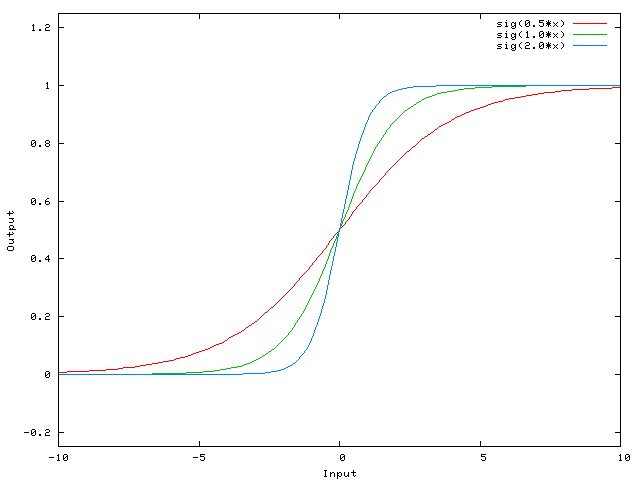
\includegraphics[scale=0.4]{images/bias.png}
        \caption{The graph of a general sigmoidal function as the coefficients 
            (weights) change. Pic taken from StackOverflow: 
            http://stackoverflow.com/questions/2480650/role-of-bias-in-neural-networks}
    \end{figure}

\subsection{How Are the Correct Weights Calculated?}

    \paragraph{}Finding the right weights is all the work. The correct weights are
    found via a process called back propagation. Back propagation is a repeated 
    process of error correction, starting with the output nodes and moving back up
    the network. The error of the output nodes is simply the difference between the
    desired output and the actual output, but the error calculation for each node 
    higher up the tree must be a summation of all collective errors of the exiting 
    connections, since each node is connected to every node in the level lower. 
    This algorithm proved to be the most difficult part of the project and I 
    consulted numerous and tutorials and open source 
    projects.\footnote{Here are some of the most helpful resources I found: \\  
    http://www.cs.montana.edu/~grayd/backprop.htm \\ 
    http://arctrix.com/nas/python/bpnn.py}
    
    \paragraph{}The network is always training in the background so the user can 
    see potentially constant improvement, and to learn more and different 
    handwriting there only needs to be more data added to the training instance 
    on the server. Also, the network takes very long to train. At the time of this 
    presentation, this network will have been training on euclid for about a 
    month, and that's not unusual. Because of the dependency on 
    adjacent layers in back propagated training, it can not be efficiently 
    parallelized\footnote{
    https://research.microsoft.com/apps/pubs/default.aspx?id=173312}.

    \paragraph{}Earlier it was mentioned that hyperbolic tangent is easily derived
    and that's nice for training. This is because we can use the derivative of the 
    activation function in calculating the weight deltas. Consider how the 
    derivative changes as the hyperbolic tangent is traveled. Since the derivative 
    is greatest at the middle -- where the activation is most uncertain -- results 
    in the middle will cause a greater change in the associated weights. 
    Conversely, as the network's weights become more established through training, 
    the derivative approaches zero and the network stabilizes.

\subsection{iOS, JSON, and CGI.}

    \paragraph{}I wanted a good way to demonstrate the working neural network. Just
    knowing it can recognize handwritten characters in a database is not very 
    exciting, but having it recognize a user's in real time would be. So an iOS 
    front end was added to take input, query the server on which the network is 
    running, and return an ordering of likeliness, from 0 to 9, of which digit it 
    was sent. The only particular I'd like to mention is how surprisingly easy it 
    was get Apache to serve Python files. A single line file in the pub directory 
    on euclid is all it takes. \\

    \begin{lstlisting}
    File: .htaccess

    AddHandler cgi-script .py
    \end{lstlisting}

\section{Software Organization...}

    \paragraph{}I chose to have an independent neural network, and I still like 
    that decision. There is nothing specific to handwriting recognition in the
    network package. What could use improvement is the way the network is 
    incorporated with the rest of the project. There are multiple applications 
    that rely on the neural network package yet it is added as a Git submodule 
    under the network training application's directory. It would be more 
    appropriate to have the Git submodule in a more neutral location and
    reference it accordingly from the other applications. 
    
    \paragraph{}There is also substantial set up to have a completely working
    demonstration (web page, network training, adding the neural network package
    to the Python Path). It would be nice to package the suite in a way that 
    facilitates a more automated out-of-the-box solution.

\section{As Hard As I Expected...}

    \paragraph{}I was expecting really hard, and it's about what I got. There were 
    a couple especially difficult hurdles as I was working on this project. When I
    first starting trying to train handwritten digit recognition I didn't
    get any performance better than about 15\% successful recognition. I trained
    network for days on even small samples of data and it just stalled. Worse 
    still, it was unpredictable and inconsistent. This is why I added the 
    "experiment" mode to the network training application. I could see that 
    "skinny" three-layer networks -- networks with fewer than about 60 nodes per 
    layer -- mastered data sets quickly and flawlessly. As the networks grew larger
    they became wildly inconsistent. The experiment trained a constant function for
    a constant number of iterations on increasingly large networks and graphed the 
    error rate and time to completion versus size. Figure~\ref{badgraph} shows the 
    inital results. There are so many moving pieces I couldn't imagine what the 
    issue was. It turns out the answer was local minima, and that turning the 
    learning and momentum rates way down would help to avoid sticking points.
    Figure~\ref{goodgraph} shows the nearly flawless performance of the improved 
    network.

    \paragraph{}The next great challenge was improving the disappointingly poor 
    performance of real life digit recognition. The network was training on euclid 
    as I was finishing the basic functionality of the iOS application, and by the 
    time I finished the logs read it was correctly recognizing more than 93\% of 
    the test data. In actual use, however, I found the network to correctly 
    interpret only the nicest of input; perfectly sized and centered submissions.
    The problem was the strict preprocessing done on the data in the MNIST Database
    did not represent unfiltered data from the real world. To improve performance,
    I "messied" up the data by changing the size and rotation. The variations I 
    added turned the training set of ~40k samples into a set of ~1.5M samples. 

    \paragraph{}The next great obstacle was the inability of a three layer network
    to learn the more complex data. After swapping the training data, the learning
    curve became stagnant at about a 70\% success rate. So I added a fourth layer.
    Similar to the bump from two to three layers, the change from three to four 
    meant lower learning rates to avoid the increased chance of becoming stuck in 
    local minima and longer training times to facilitate the exponentially 
    increasing number of connections. Alas, it seems to be working with acceptable
    performance. To further increase the performance, I believe finding an 
    appropriate bounding box per submitted sample on the iOS application would 
    yield noticable improvements.

    \begin{figure}
        \centering
        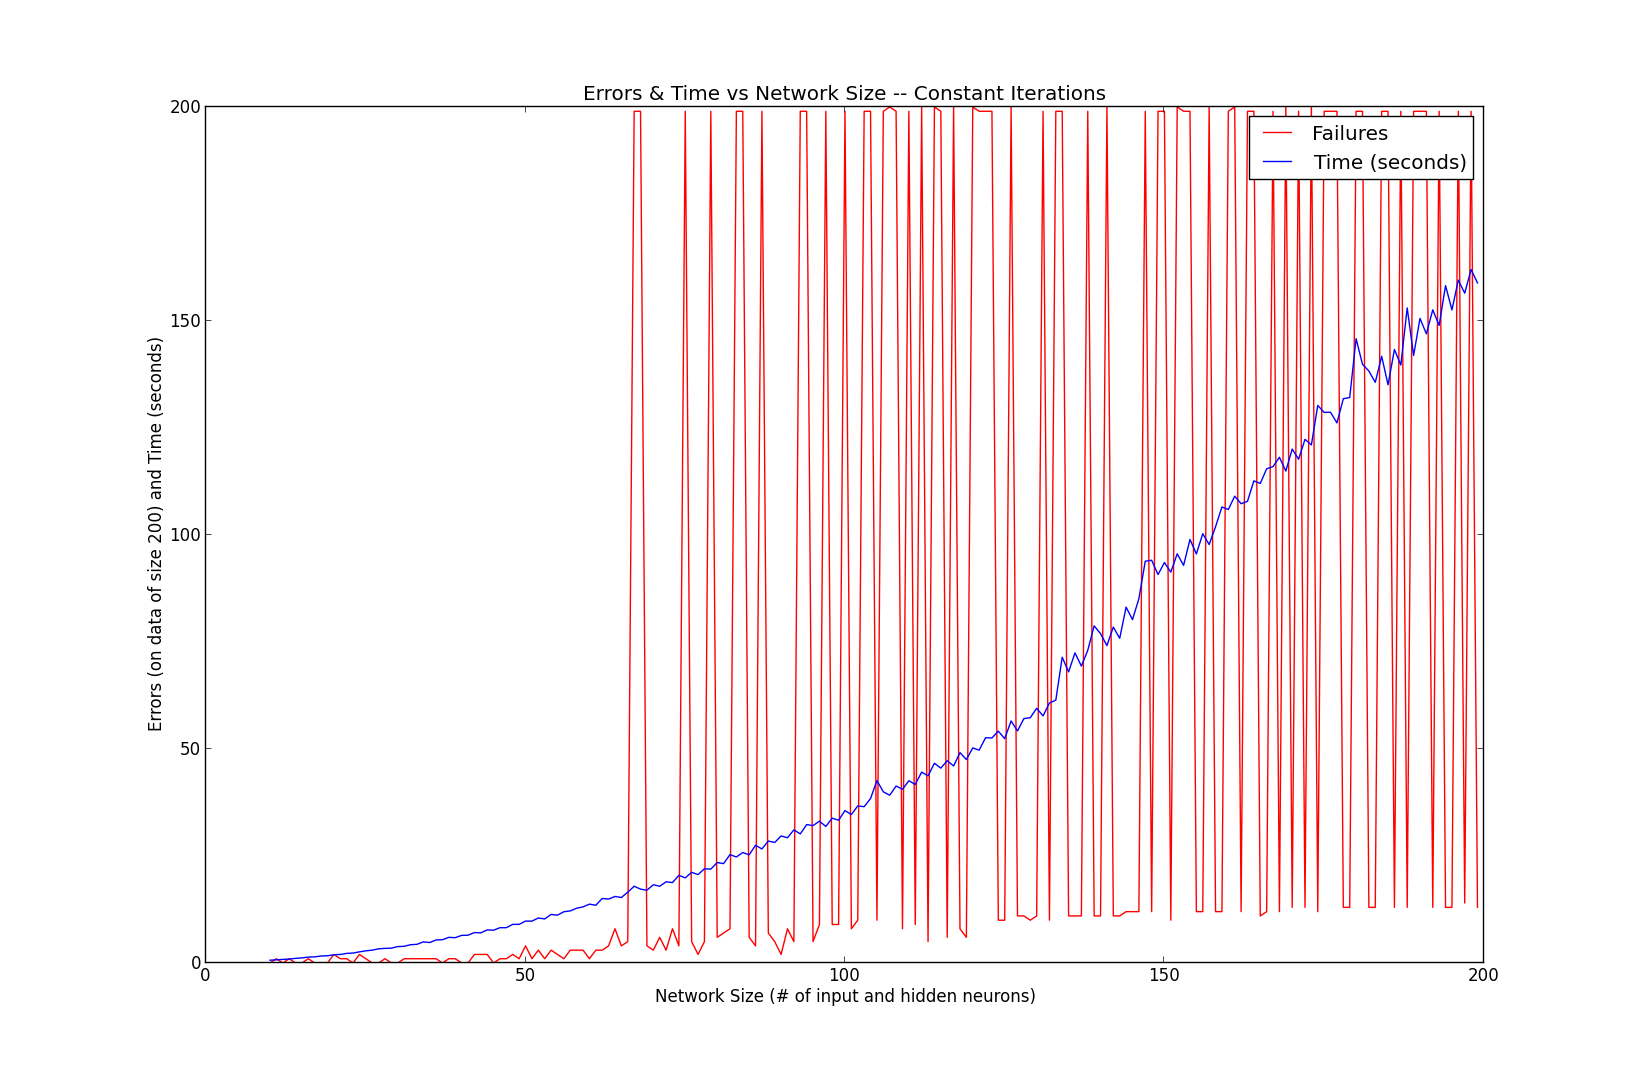
\includegraphics[scale=0.4]{images/bad_learning.png}
        \caption{The experiment run with the initial learning rate. Notice that
            as the network grows larger the success of the network becomes as
            unsure as a coin flip.}
        \label{badgraph}
    \end{figure}

    \begin{figure}
        \centering
        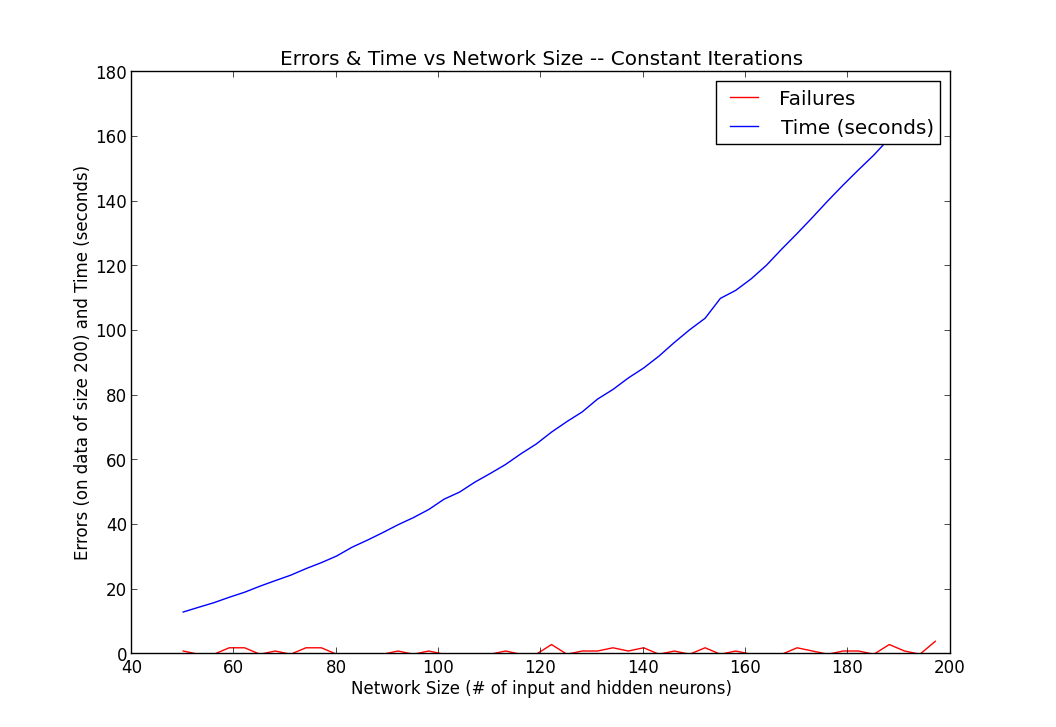
\includegraphics[scale=0.5]{images/good_learning.png}
        \caption{The experiment run with a learning rate and momentum rate 
            1/1000th the magnitude of that used in Figure~\ref{badgraph}}
        \label{goodgraph}
    \end{figure}

    \paragraph{}Here are the approximate line 
    counts\footnote{iOS App is forked from GLPaint by Apple: 
    https://developer.apple.com/library/ios/\#samplecode/GLPaint/}. \\

    \begin{tabular}{ l c r }
        Part & Line Count & Language \\
        \hline \\
        Neural Network & 542 & Python \\
        Network Training & 1142 & Python \\
        Web Site & 67 & Python \\
        iOS App & 1564 & Objective C \\
        Total & 3315 & All \\
    \end{tabular}

\end{document}
